\documentclass[conference]{IEEEtran}
\IEEEoverridecommandlockouts
% The preceding line is only needed to identify funding in the first footnote. If that is unneeded, please comment it out.
\usepackage{cite}
\usepackage{algorithm}
\usepackage{amsmath,amssymb,amsfonts}
\usepackage{algorithmic}
\usepackage{graphicx}
\usepackage{textcomp}
\usepackage{physics}
\usepackage{amsmath}% http://ctan.org/pkg/amsmath
\newcommand\sufr[3][0pt]{$\rule{0pt}{\dimexpr#1+1.4ex\relax}^\frac{#2}{#3}$}
\usepackage{xcolor}
\def\BibTeX{{\rm B\kern-.05em{\sc i\kern-.025em b}\kern-.08em
    T\kern-.1667em\lower.7ex\hbox{E}\kern-.125emX}}
\begin{document}

\title{Quantum Mechanics Enabled Genetic Programming\\
% {\footnotesize \textsuperscript{*}Note: Sub-titles are not captured in Xplore and
% should not be used}
% \thanks{Identify applicable funding agency here. If none, delete this.}
}

% \author{\IEEEauthorblockN{1\textsuperscript{st} Given Name Surname}
% \IEEEauthorblockA{\textit{dept. name of organization (of Aff.)} \\
% \textit{name of organization (of Aff.)}\\
% City, Country \\
% email address}
% \and
% \IEEEauthorblockN{2\textsuperscript{nd} Given Name Surname}
% \IEEEauthorblockA{\textit{dept. name of organization (of Aff.)} \\
% \textit{name of organization (of Aff.)}\\
% City, Country \\
% email address}
% \and
% \IEEEauthorblockN{3\textsuperscript{rd} Given Name Surname}
% \IEEEauthorblockA{\textit{dept. name of organization (of Aff.)} \\
% \textit{name of organization (of Aff.)}\\
% City, Country \\
% email address}
% \and
% \IEEEauthorblockN{4\textsuperscript{th} Given Name Surname}
% \IEEEauthorblockA{\textit{dept. name of organization (of Aff.)} \\
% \textit{name of organization (of Aff.)}\\
% City, Country \\
% email address}
% \and
% \IEEEauthorblockN{5\textsuperscript{th} Given Name Surname}
% \IEEEauthorblockA{\textit{dept. name of organization (of Aff.)} \\
% \textit{name of organization (of Aff.)}\\
% City, Country \\
% email address}
% \and
% \IEEEauthorblockN{6\textsuperscript{th} Given Name Surname}
% \IEEEauthorblockA{\textit{dept. name of organization (of Aff.)} \\
% \textit{name of organization (of Aff.)}\\
% City, Country \\
% email address}
% }

\maketitle

\begin{abstract}
Quantum Computing (QC) has often been touted as an esoteric and terrifying field of computing research. However, the possible advantages offered by the inherent quantum fundamentals beseeches extensive additional ventures into this field. Just as QP offers exciting ideas in the field of computing, Genetic Programming (GP) offers an application oriented optimization route. GP uses Darwinian theories to maintain a set of candidate solutions, apply multiple operations on the candidates and eventually declare a global winner. In this paper, we combine QC and a flavour of GP to create a new interdisciplinary front of computational intelligence. 
\end{abstract}

\begin{IEEEkeywords}
component, formatting, style, styling, insert
\end{IEEEkeywords}

\section{Introduction}

Majority of the problems faced in any aspect of computer science, in one way or another, involves a catch-22 of multi-functional optimization. Entire fields have been dedicated to solving a generic version of this issue. The most common method of dealing with optimization problems is to be in collaboration with another interdisciplinary frontier acting in the capacity of a helper function. 


\subsection{Computing Methodologies}

Most form of computational algorithms in the present day, are executed on a conventional computer. The fundamental notation used for differentiating Classical Computing (CC) and QC is the basic unit of information. While classical computers use bits 0 and 1, quantum computers use "one of" two computational basis states. The label awarded to these states is "bra-ket" notation i.e, state $\ket{0}$ or $\ket{1}$. Bits are assigned states 0 or 1 deterministically and independently. However, qbuits can exist in a superposition state of $\alpha\textsubscript{0}$$\ket{0}$ + $\alpha\textsubscript{1}$$\ket{1}$, where $\alpha{0}$ and $\alpha{1}$ are complex numbers, such that $|\alpha\textsubscript{0}|\textsuperscript{2}$ + $|\alpha\textsubscript{1}|\textsuperscript{2}$ = 1.

\subsection{Why go Quantum?}

The field of applied quantum mechanics is still unexplored for the best part. However, there are certain applications in which QC outperforms CC. Consider Shor's algorithm and RSA, both of which are used for encryption. Basically, the encryption of any form of data transmitted over the Internet relies immensley on factorization of a huge number. This process is extremley ardous for a non-quantum computer, with the best known factoring technique requiring an amount of time proportional to 2$\textsuperscript{n\textsuperscript{\sufr{1}{3}}log(n)\textsuperscript{\sufr{2}{3}}}$ 
, where $\textit{n}$ is the number of digits in the number to be factored. Meanwhile Shor's Quantum algorithm requires time proportional to only $n\textsuperscript{2}log(n)log(log(n))$. 

QC takes advantage of major quantum phenomena such as superposition, quantum entanglment, principle of uncertainity among others, for improving existing searchc and optimization techniques. Humans inherently stick to definitive physical concepts such as deterministic state transition, state duality and temporal static behaviour of particles. 

According to Moore's Law, the size of computational units shrinks at an exponential rate as the number of transistors on a chipset increases every year. Even after accounting for physical constraints, a time will come when operations will be conducted on an atomic scale. On such a level, atomic forces overpower particle physics naturally. As a result, understanding QC and applying them in a virtual landscape to get a sense of their possibilities is a must. 

\subsection{Using Evolutionary Algorithms}

Evolutionary Algorithms (EA) encompass a wide array of research ideas stemming from general principles of genetics and the theory of evolution. Models are developed to illustrate the behaviour of naturally occuring phenomena, develop these algorithms and test out the application of the corresponding theory. The general process of any EA is depicted in figure \ref{p1}. In a nutshell, an initial population of candidate solutions is generated and each solution is labelled according to their performance on a set fitness function. Further down the line, these candidates are improved upon by conducting a set of operations on them for a predetermined number of generations. After some stopping criterias are achieved, the process strops and the best candidate is hypothesized as the global solution. The advantages offered by this technqiue include but not limited to resilience to noise, in-built support for parallelism and distributed learning, multi-pronged attack and handling complex problems. 

\begin{figure}[!t]
\centering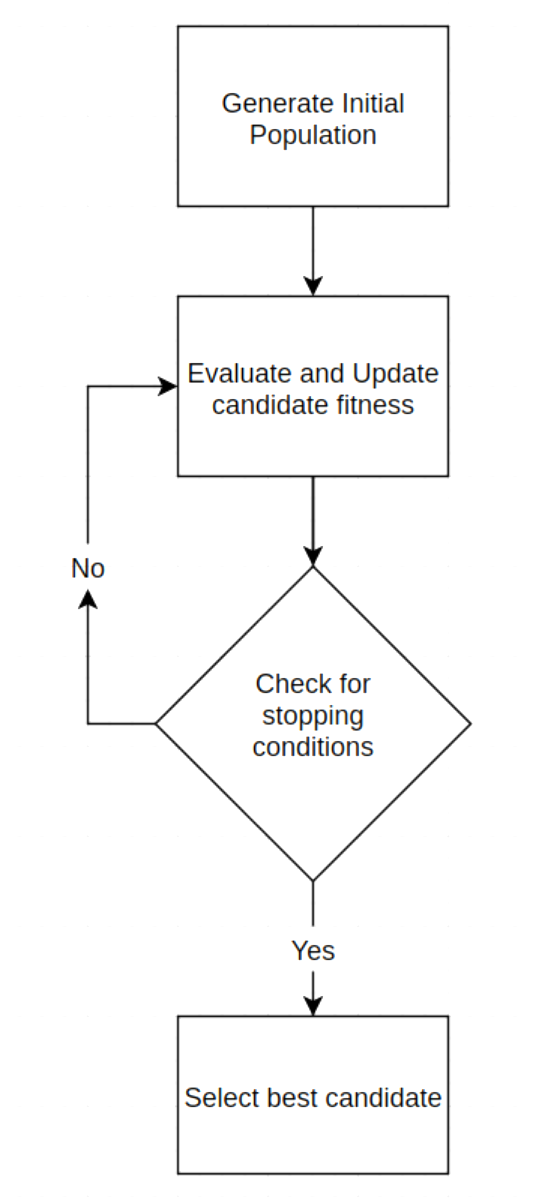
\includegraphics[height=6.75cm]{p1.png}
\caption{General Flow of Evolutionary Algorithms}
\label{p1}
\end{figure}

Our paper provides an insight into the ensemble of both the previously mentioned techniques and preparing algorithms for a future where quantum computers replace traditional computers as commonplace machines. 

\section{Methodology}

One of the most famous quantum effect invovles "superposition", which allows a quantum entity to exist simultaneously. As a result memory conservation capabilities of any quantum system increases exponentially. Coupling this idea with multiple evolutionary aspects, we present a novel computational frontier. 

\subsection{Existing Convention}

Consider the following problem; Assume the position of a process $\textit{P}$ in a finite state system of $\textit{n}$ states at time $\textit{t}$ to be $\textit{x\textsubscript{i}}$. Create a general procedure to reach position $\textit{x\textsubscript{j}}$ at time $\textit{t+1}$.

The conventional process would involve declaration of a register of size $\textit{n}$ and listing out all possible combinations for reaching state $\textit{x\textsubscript{j}}$ along with the costs. This would be followed by creation of a logical circutry of gates mapping the input state to the output state using boolean primitives. The entire process could still be automated using certain advanced algorithms. However, the memory utilization will not be optimal as all possible state transitions must be considered before building the circuit. Figure $\ref{p2}$ displays the state table, state diagram and accompanying circuit diagram for a D flip flop. Notice that all possible states for the input have been mentioned in the state table. This constitues a huge waste of memory as majority of the inputs are never encountered and some states could be invalid. QC aims to reduce this inefficiency between making all the states dependent on each other. 

\begin{figure}[!b]
\centering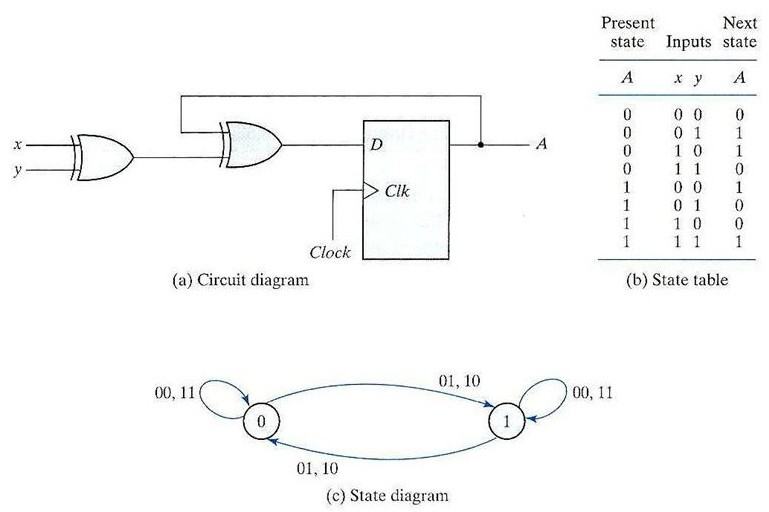
\includegraphics[width=8cm]{ss.jpg}
\caption{States for D flip flop}
\label{p2}
\end{figure}

\subsection{Applied Quantum Mechanics}
Classicial state transitions cannot fathom superposition and hence will always be fixated on one fixed state. For the D flip flop example, the number of inputs are two and hence the number of output states is $2\textsuperscript{2}$ for each starting state. The 4 possible states can be represented as an one-hot encoded vector with each bit representing the state of the output. For example, the vector shown below represents state 00 for an input state of 0.
$$
\begin{bmatrix} 
1&0&0&0\\
\end{bmatrix}
\quad
$$

Quantum Mechanics is a generalized extension of classical method. The first generalization comes in the form of the temporal values of the elements of the matrix. In QC qubits are utilized instead of bits and as a result the state vectors are variables. Instead of 0 and 1, state vector can be constituted of complex numbers which meet the condition of unitarity. For any matrix $\textit{M}$ to be an unitarity matrix, the only necessary condition is shown in Equation $\ref{eq:1}$ where $M\textsuperscript{$\dagger$}$ is the Hermitean adjoint of $\textit{M}$ and $\textit{I}$ is the identity matrix. 

\begin{equation}
\label{eq:1}
M\textsuperscript{$\dagger$}M = MM\textsuperscript{$\dagger$} = I
\end{equation}

To facilitate the design of circuitry of state diagrams, QC introduces a set of gates to utilize the power of quantum mechanics. The noteworthy ones are mentioned below:

\begin{itemize}
\item QNOT: This gate is the quantum extension of the controlled NOT gate in CC. A controlled NOT gate performs the inversion operation on the right-most bit of a vector iff the left-most bit is 1. A 1-bit QNOT gate is depicted as follows:
$$
\begin{bmatrix} 
0&1\\
1&0\\
\end{bmatrix}
\quad
$$
\item SRN: The application of Square Root of NOT puts a qubit into a state of equal superposition through controlled randomization based on the qubit's past state. A 1-bit SRN is shown below:
$$
\begin{bmatrix} 
\frac{1}{\sqrt{2}}&\frac{-1}{\sqrt{2}}\\
\frac{1}{\sqrt{2}}&\frac{1}{\sqrt{2}}\\
\end{bmatrix}
\quad
$$
\item Swap: As the name suggests, this gate is used to swap the states of two qubits and is represented as:
$$
\begin{bmatrix} 
{1}&{0}&{0}&{0}\\
{0}&{0}&{1}&{0}\\
{0}&{1}&{0}&{0}\\
{0}&{0}&{0}&{1}\\
\end{bmatrix}
\quad
$$
\item Parameterized Rotation: This is a family of 1-qubit rotations parameterized by angle $\theta$ and is given by:
$$
\begin{bmatrix} 
cos(\theta)&sin(\theta)\\
-sin(\theta)&cos(\theta)\\
\end{bmatrix}
\quad
$$
\end{itemize}

\subsection{Applied Evolutionary Operators}

EA have been used extensively for complex optimization problems due to quality results even with a lack of mathematical representation, convexity and continuity. They apply a stochastic method and hence expedite the search process. However, EA are not without their flaws which include a probabilistic convergence to the global optima. 

In this paper, we follow a genetic modified Grey Wolf Optimization (GWO) algorithm to obtain and update candidate solutions. GWO follows a hierarchical structure of candidate solution which imitates the behaviour of Grey Wolves as observed in nature. The structure of $\alpha$, $\beta$, $\delta$ and $\omega$ labelled wolves. The $\alpha$ wolves are responsible for finding the global optimum whilst being guided by the $\beta$ wolves. The $\delta$ and $\omega$ provide secondary assistance to the leaders and hence maitain the dominant structure. After each search iteration, genetic operators like selection, crossover and mutation are applied to every candidate in the structure. The entire process is discribed in Algorithm $\ref{alg:gwo}$

\begin{algorithm}[t]
\footnotesize
\caption{GWO pseudocode}
\label{alg:gwo}
\begin{algorithmic}[1]
\STATE \textbf{Input:} Population size $\textit{n}$, random vectors $\vec{r\textsubscript{1}}$, $\vec{r\textsubscript{2}} \in$ [0,1], initial prey location $\vec{D}$, number of iterations \textit{I}, fitness function $\textit{f}$, coefficient vectors $\vec{A}$, $\vec{C}$ and $\vec{a}$
\STATE Set $\textit{t}$ = 0
\FOR{i $\in$ [1,n]}    
\STATE Generate wolf pack population $\textit{X\textsubscript{i}(t)}$ at instance $\textit{t}$
\STATE Evaluate each individual against the fitness function
\ENDFOR
\STATE Assign $\alpha, \beta, \delta$ titles to the top three solutions
\STATE Evaluate $\vec{D} = |\vec{C} \cdot \vec{X\textsubscript{p}}(t) - \vec{X}(t)|$
\FOR{\textit{i} in \textit{I}}
\FOR{Each individual in $\textit{n}$}  
\STATE $\vec{X\textsubscript{1}} = \vec{X\textsubscript{$\alpha$}} - \vec{A\textsubscript{1}} \cdot  \vec{D\textsubscript{$\alpha$}}$
\STATE $\vec{X\textsubscript{2}} = \vec{X\textsubscript{$\beta$}} - \vec{A\textsubscript{2}} \cdot  \vec{D\textsubscript{$\beta$}}$
\STATE $\vec{X\textsubscript{3}} = \vec{X\textsubscript{$\delta$}} - \vec{A\textsubscript{3}} \cdot  \vec{D\textsubscript{$\delta$}}$
\STATE Evaluate $\vec{X}(t+1) = \frac{\vec{X\textsubscript{1}} + \vec{X\textsubscript{2}} + \vec{X\textsubscript{3}}}{3}$
\ENDFOR
\STATE Update the coefficient vectors $\vec{A}$ and $\vec{C}$
\STATE $\vec{A} = 2\vec{a} \cdot \vec{r\textsubscript{1}} - \vec{a}$
\STATE $\vec{C} = 2\vec{r\textsubscript{2}}$
\STATE Linearly decrease $\vec{a}$ from 2 to 0
% \STATE Update $\vec{X\textsubscript{$\alpha$}}, \vec{X\textsubscript{$\beta$}}, \vec{X\textsubscript{$\delta$}}$
\STATE Perform Crossover, Selection and Mutation
\STATE Increment $\textit{t}$
\ENDFOR
\STATE $\vec{X\textsubscript{$\alpha$}}$ corresponds to the global optimum. 
\end{algorithmic}
\end{algorithm}

The genetic operators for a sample candidate in the form of a genomic are explained here following which the process is depicted in Figure :
\begin{itemize}
\item Selection: Given a population of potential solutions, selection involves grading these solutions against a fitness function. The selected solutions are cast into the crossover stage.
\item Crossover: From the selected set of solutions, randomly two solutions are selected and the next generation chromosome is created which shares the best attributes of it's parents.
\item Mutation: The selected solutions undergo random changes in their composition to promote diversity and increase their changes of converging to the global optimum.
\end{itemize}

\begin{figure}
\centering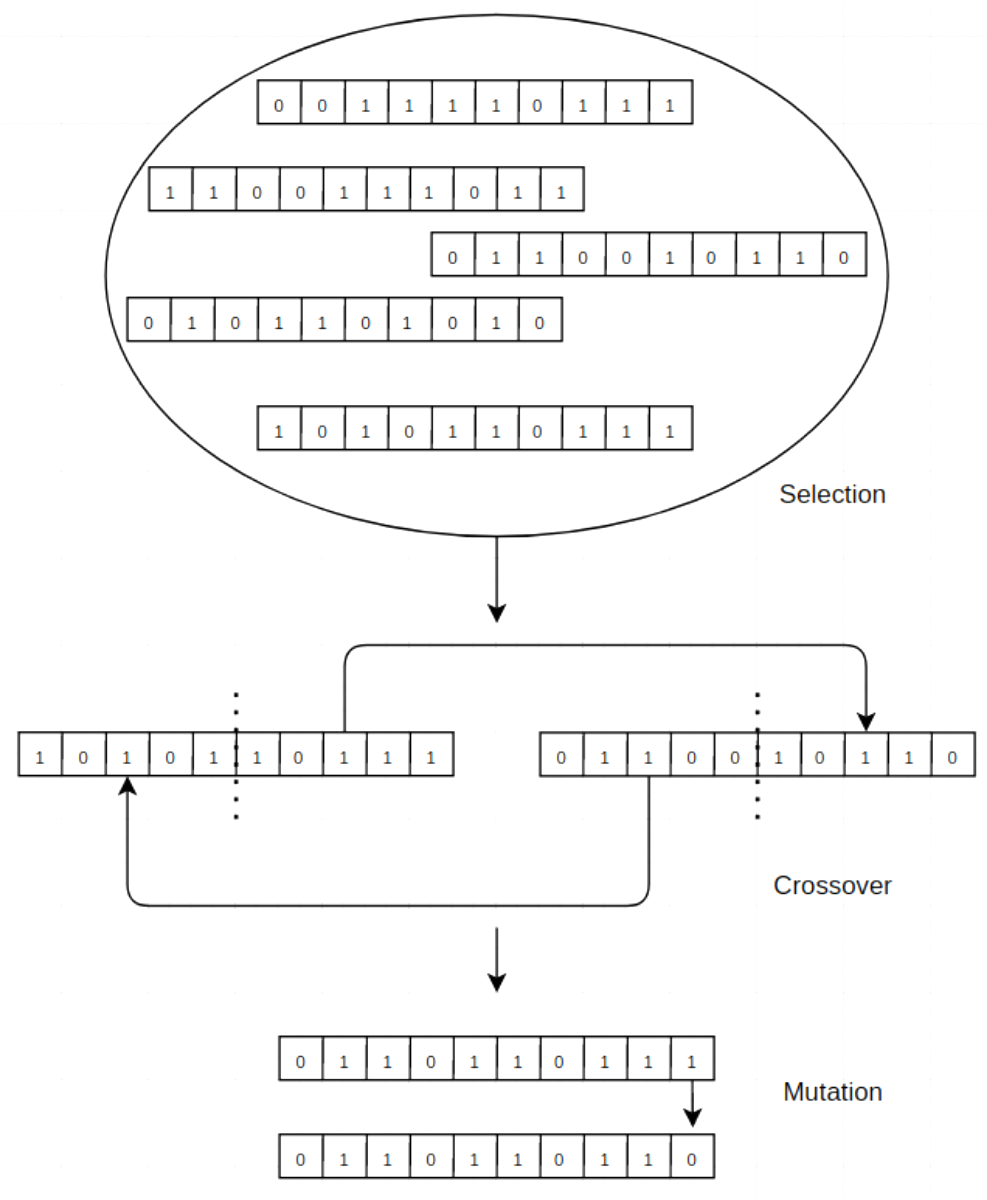
\includegraphics[width=7cm]{p2.png}
\caption{Genetic Operators}
\label{p3}
\end{figure}
% This document is a model and instructions for \LaTeX.
% Please observe the conference page limits. 
% 
% \section{Ease of Use}
% 
% \subsection{Maintaining the Integrity of the Specifications}
% 
% The IEEEtran class file is used to format your paper and style the text. All margins, 
% column widths, line spaces, and text fonts are prescribed; please do not 
% alter them. You may note peculiarities. For example, the head margin
% measures proportionately more than is customary. This measurement 
% and others are deliberate, using specifications that anticipate your paper 
% as one part of the entire proceedings, and not as an independent document. 
% Please do not revise any of the current designations.
% 
% \section{Prepare Your Paper Before Styling}
% Before you begin to format your paper, first write and save the content as a 
% separate text file. Complete all content and organizational editing before 
% formatting. Please note sections \ref{AA}--\ref{SCM} below for more information on 
% proofreading, spelling and grammar.
% 
% Keep your text and graphic files separate until after the text has been 
% formatted and styled. Do not number text heads---{\LaTeX} will do that 
% for you.
% 
% \subsection{Abbreviations and Acronyms}\label{AA}
% Define abbreviations and acronyms the first time they are used in the text, 
% even after they have been defined in the abstract. Abbreviations such as 
% IEEE, SI, MKS, CGS, ac, dc, and rms do not have to be defined. Do not use 
% abbreviations in the title or heads unless they are unavoidable.
% 
% \subsection{Units}
% \begin{itemize}
% \item Use either SI (MKS) or CGS as primary units. (SI units are encouraged.) English units may be used as secondary units (in parentheses). An exception would be the use of English units as identifiers in trade, such as ``3.5-inch disk drive''.
% \item Avoid combining SI and CGS units, such as current in amperes and magnetic field in oersteds. This often leads to confusion because equations do not balance dimensionally. If you must use mixed units, clearly state the units for each quantity that you use in an equation.
% \item Do not mix complete spellings and abbreviations of units: ``Wb/m\textsuperscript{2}'' or ``webers per square meter'', not ``webers/m\textsuperscript{2}''. Spell out units when they appear in text: ``. . . a few henries'', not ``. . . a few H''.
% \item Use a zero before decimal points: ``0.25'', not ``.25''. Use ``cm\textsuperscript{3}'', not ``cc''.)
% \end{itemize}
% 
% \subsection{Equations}
% Number equations consecutively. To make your 
% equations more compact, you may use the solidus (~/~), the exp function, or 
% appropriate exponents. Italicize Roman symbols for quantities and variables, 
% but not Greek symbols. Use a long dash rather than a hyphen for a minus 
% sign. Punctuate equations with commas or periods when they are part of a 
% sentence, as in:
% \begin{equation}
% a+b=\gamma\label{eq}
% \end{equation}
% 
% Be sure that the 
% symbols in your equation have been defined before or immediately following 
% the equation. Use ``\eqref{eq}'', not ``Eq.~\eqref{eq}'' or ``equation \eqref{eq}'', except at 
% the beginning of a sentence: ``Equation \eqref{eq} is . . .''
% 
% \subsection{\LaTeX-Specific Advice}
% 
% Please use ``soft'' (e.g., \verb|\eqref{Eq}|) cross references instead
% of ``hard'' references (e.g., \verb|(1)|). That will make it possible
% to combine sections, add equations, or change the order of figures or
% citations without having to go through the file line by line.
% 
% Please don't use the \verb|{eqnarray}| equation environment. Use
% \verb|{align}| or \verb|{IEEEeqnarray}| instead. The \verb|{eqnarray}|
% environment leaves unsightly spaces around relation symbols.
% 
% Please note that the \verb|{subequations}| environment in {\LaTeX}
% will increment the main equation counter even when there are no
% equation numbers displayed. If you forget that, you might write an
% article in which the equation numbers skip from (17) to (20), causing
% the copy editors to wonder if you've discovered a new method of
% counting.
% 
% {\BibTeX} does not work by magic. It doesn't get the bibliographic
% data from thin air but from .bib files. If you use {\BibTeX} to produce a
% bibliography you must send the .bib files. 
% 
% {\LaTeX} can't read your mind. If you assign the same label to a
% subsubsection and a table, you might find that Table I has been cross
% referenced as Table IV-B3. 
% 
% {\LaTeX} does not have precognitive abilities. If you put a
% \verb|\label| command before the command that updates the counter it's
% supposed to be using, the label will pick up the last counter to be
% cross referenced instead. In particular, a \verb|\label| command
% should not go before the caption of a figure or a table.
% 
% Do not use \verb|\nonumber| inside the \verb|{array}| environment. It
% will not stop equation numbers inside \verb|{array}| (there won't be
% any anyway) and it might stop a wanted equation number in the
% surrounding equation.
% 
% \subsection{Some Common Mistakes}\label{SCM}
% \begin{itemize}
% \item The word ``data'' is plural, not singular.
% \item The subscript for the permeability of vacuum $\mu_{0}$, and other common scientific constants, is zero with subscript formatting, not a lowercase letter ``o''.
% \item In American English, commas, semicolons, periods, question and exclamation marks are located within quotation marks only when a complete thought or name is cited, such as a title or full quotation. When quotation marks are used, instead of a bold or italic typeface, to highlight a word or phrase, punctuation should appear outside of the quotation marks. A parenthetical phrase or statement at the end of a sentence is punctuated outside of the closing parenthesis (like this). (A parenthetical sentence is punctuated within the parentheses.)
% \item A graph within a graph is an ``inset'', not an ``insert''. The word alternatively is preferred to the word ``alternately'' (unless you really mean something that alternates).
% \item Do not use the word ``essentially'' to mean ``approximately'' or ``effectively''.
% \item In your paper title, if the words ``that uses'' can accurately replace the word ``using'', capitalize the ``u''; if not, keep using lower-cased.
% \item Be aware of the different meanings of the homophones ``affect'' and ``effect'', ``complement'' and ``compliment'', ``discreet'' and ``discrete'', ``principal'' and ``principle''.
% \item Do not confuse ``imply'' and ``infer''.
% \item The prefix ``non'' is not a word; it should be joined to the word it modifies, usually without a hyphen.
% \item There is no period after the ``et'' in the Latin abbreviation ``et al.''.
% \item The abbreviation ``i.e.'' means ``that is'', and the abbreviation ``e.g.'' means ``for example''.
% \end{itemize}
% An excellent style manual for science writers is \cite{b7}.
% 
% \subsection{Authors and Affiliations}
% \textbf{The class file is designed for, but not limited to, six authors.} A 
% minimum of one author is required for all conference articles. Author names 
% should be listed starting from left to right and then moving down to the 
% next line. This is the author sequence that will be used in future citations 
% and by indexing services. Names should not be listed in columns nor group by 
% affiliation. Please keep your affiliations as succinct as possible (for 
% example, do not differentiate among departments of the same organization).
% 
% \subsection{Identify the Headings}
% Headings, or heads, are organizational devices that guide the reader through 
% your paper. There are two types: component heads and text heads.
% 
% Component heads identify the different components of your paper and are not 
% topically subordinate to each other. Examples include Acknowledgments and 
% References and, for these, the correct style to use is ``Heading 5''. Use 
% ``figure caption'' for your Figure captions, and ``table head'' for your 
% table title. Run-in heads, such as ``Abstract'', will require you to apply a 
% style (in this case, italic) in addition to the style provided by the drop 
% down menu to differentiate the head from the text.
% 
% Text heads organize the topics on a relational, hierarchical basis. For 
% example, the paper title is the primary text head because all subsequent 
% material relates and elaborates on this one topic. If there are two or more 
% sub-topics, the next level head (uppercase Roman numerals) should be used 
% and, conversely, if there are not at least two sub-topics, then no subheads 
% should be introduced.
% 
% \subsection{Figures and Tables}
% \paragraph{Positioning Figures and Tables} Place figures and tables at the top and 
% bottom of columns. Avoid placing them in the middle of columns. Large 
% figures and tables may span across both columns. Figure captions should be 
% below the figures; table heads should appear above the tables. Insert 
% figures and tables after they are cited in the text. Use the abbreviation 
% ``Fig.~\ref{fig}'', even at the beginning of a sentence.
% 
% \begin{table}[htbp]
% \caption{Table Type Styles}
% \begin{center}
% \begin{tabular}{|c|c|c|c|}
% \hline
% \textbf{Table}&\multicolumn{3}{|c|}{\textbf{Table Column Head}} \\
% \cline{2-4} 
% \textbf{Head} & \textbf{\textit{Table column subhead}}& \textbf{\textit{Subhead}}& \textbf{\textit{Subhead}} \\
% \hline
% copy& More table copy$^{\mathrm{a}}$& &  \\
% \hline
% \multicolumn{4}{l}{$^{\mathrm{a}}$Sample of a Table footnote.}
% \end{tabular}
% \label{tab1}
% \end{center}
% \end{table}
% 
% % \begin{figure}[htbp]
% % \centerline{\includegraphics{fig1.png}}
% % \caption{Example of a figure caption.}
% % \label{fig}
% % \end{figure}
% 
% Figure Labels: Use 8 point Times New Roman for Figure labels. Use words 
% rather than symbols or abbreviations when writing Figure axis labels to 
% avoid confusing the reader. As an example, write the quantity 
% ``Magnetization'', or ``Magnetization, M'', not just ``M''. If including 
% units in the label, present them within parentheses. Do not label axes only 
% with units. In the example, write ``Magnetization (A/m)'' or ``Magnetization 
% \{A[m(1)]\}'', not just ``A/m''. Do not label axes with a ratio of 
% quantities and units. For example, write ``Temperature (K)'', not 
% ``Temperature/K''.
% 
% \section*{Acknowledgment}
% 
% The preferred spelling of the word ``acknowledgment'' in America is without 
% an ``e'' after the ``g''. Avoid the stilted expression ``one of us (R. B. 
% G.) thanks $\ldots$''. Instead, try ``R. B. G. thanks$\ldots$''. Put sponsor 
% acknowledgments in the unnumbered footnote on the first page.
% 
% \section*{References}
% 
% Please number citations consecutively within brackets \cite{b1}. The 
% sentence punctuation follows the bracket \cite{b2}. Refer simply to the reference 
% number, as in \cite{b3}---do not use ``Ref. \cite{b3}'' or ``reference \cite{b3}'' except at 
% the beginning of a sentence: ``Reference \cite{b3} was the first $\ldots$''
% 
% Number footnotes separately in superscripts. Place the actual footnote at 
% the bottom of the column in which it was cited. Do not put footnotes in the 
% abstract or reference list. Use letters for table footnotes.
% 
% Unless there are six authors or more give all authors' names; do not use 
% ``et al.''. Papers that have not been published, even if they have been 
% submitted for publication, should be cited as ``unpublished'' \cite{b4}. Papers 
% that have been accepted for publication should be cited as ``in press'' \cite{b5}. 
% Capitalize only the first word in a paper title, except for proper nouns and 
% element symbols.
% 
% For papers published in translation journals, please give the English 
% citation first, followed by the original foreign-language citation \cite{b6}.
% 

% \begin{thebibliography}{00}
% \bibitem{chankong} Chankong V., Haimes Y, Thadathil J., Zionts S. (1985), Multiple Criteria Optimization: A State of the Art Review, Decision Making with Multiple Objectives, Lecture Notes in Economics and Mathematical Systems 242, Edited by Y.Y. Haimes, V. Chankong, SpringerVerlag, 36.
% \end{thebibliography}

% \begin{thebibliography}{00}
% \bibitem{b1} G. Eason, B. Noble, and I. N. Sneddon, ``On certain integrals of Lipschitz-Hankel type involving products of Bessel functions,'' Phil. Trans. Roy. Soc. London, vol. A247, pp. 529--551, April 1955.
% \bibitem{b2} J. Clerk Maxwell, A Treatise on Electricity and Magnetism, 3rd ed., vol. 2. Oxford: Clarendon, 1892, pp.68--73.
% \bibitem{b3} I. S. Jacobs and C. P. Bean, ``Fine particles, thin films and exchange anisotropy,'' in Magnetism, vol. III, G. T. Rado and H. Suhl, Eds. New York: Academic, 1963, pp. 271--350.
% \bibitem{b4} K. Elissa, ``Title of paper if known,'' unpublished.
% \bibitem{b5} R. Nicole, ``Title of paper with only first word capitalized,'' J. Name Stand. Abbrev., in press.
% \bibitem{b6} Y. Yorozu, M. Hirano, K. Oka, and Y. Tagawa, ``Electron spectroscopy studies on magneto-optical media and plastic substrate interface,'' IEEE Transl. J. Magn. Japan, vol. 2, pp. 740--741, August 1987 [Digests 9th Annual Conf. Magnetics Japan, p. 301, 1982].
% \bibitem{b7} M. Young, The Technical Writer's Handbook. Mill Valley, CA: University Science, 1989.
% \end{thebibliography}
% \vspace{12pt}
% \color{red}
% IEEE conference templates contain guidance text for composing and formatting conference papers. Please ensure that all template text is removed from your conference paper prior to submission to the conference. Failure to remove the template text from your paper may result in your paper not being published.

\end{document}
